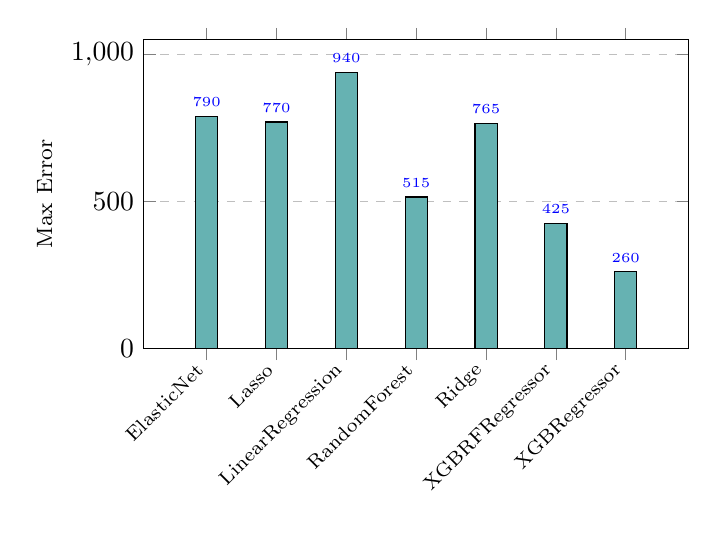
\begin{tikzpicture}
    \begin{axis}[
        ybar,
        % 1. COMPACT DIMENSIONS
        width=8.5cm,   % Significantly reduced width
        height=5.5cm,  % Reduced height
        bar width=8pt, % Slimmer bars to fit the smaller width
        % 2. TIGHTER LIMITS
        enlarge x limits=0.15, % Reduces white space on left/right edges
        ymin=0, ymax=1050,     % Tightened Y-axis slightly
        ylabel={Max Error},
        ylabel style={font=\footnotesize}, % Smaller label font
        symbolic x coords={
            ElasticNet, Lasso, LinearRegression, RandomForest, 
            Ridge, XGBRFRegressor, XGBRegressor
        },
        xtick=data,
        % 3. COMPACT LABELS
        xticklabel style={
            rotate=45, 
            anchor=east, 
            font=\scriptsize % Smaller text for model names
        },
        ymajorgrids=true,
        grid style=dashed,
        nodes near coords,
        nodes near coords style={font=\tiny}, % Tiny font for numbers on bars
    ]
    \addplot+[fill=teal!60, draw=black] coordinates {
        (ElasticNet, 790)
        (Lasso, 770)
        (LinearRegression, 940)
        (RandomForest, 515)
        (Ridge, 765)
        (XGBRFRegressor, 425)
        (XGBRegressor, 260)
    };
    
    \end{axis}
\end{tikzpicture}